\documentclass[16pt]{article}
 
% Preamble

\usepackage[margin=22mm]{geometry}
\usepackage{amsfonts, amsmath, amssymb}
\usepackage{fancyhdr, float, graphicx}
\usepackage[utf8]{inputenc} % Required for inputting international characters
\usepackage[T1]{fontenc} % Output font encoding for international characters
\usepackage{fouriernc} % Use the New Century Schoolbook font
\usepackage[nottoc, notlot, notlof]{tocbibind}
\usepackage{listings}
% \usepackage{url}
% \usepackage[options]{karnaugh-map}
% \usepackage{luacode}
% Header and Footer
\pagestyle{fancy}
\fancyhead{}
\fancyfoot{}
\fancyhead[L]{\textit{\Large{Assignment 1}}}
\fancyhead[R]{\textit{SET}}
\fancyfoot[C]{\thepage}
\renewcommand{\footrulewidth}{1pt}

% Other Doc Editing
% \parindent 0ex
%\renewcommand{\baselinestretch}{1.5}

\begin{document}

\begin{titlepage}
	\centering

	%---------------------------NAMES-------------------------------

	\huge\textsc{
		MIT World Peace University
	}\\

	\vspace{1\baselineskip} % space after Uni Name

	\LARGE{
		Software Engineering and Testing\\
		Second Year B.Tech, Semester 2
	}

	\vfill % space after Sub Name

	%--------------------------TITLE-------------------------------

	% \rule{\textwidth}{1.6pt}\vspace*{-\baselineskip}\vspace*{2pt}
	% \rule{\textwidth}{0.6pt}
	\vspace{1\baselineskip} % Whitespace above the title



	\huge{\textsc{
        PERFORMING SECURE SYSTEMS
        ANALYSIS AND DESIGN
        DRAWING DATA FLOW DIAGRAMS (LEVEL 0, 1, 2)
		}} \\



	% \vspace{0.5\baselineskip} % Whitespace below the title
	% \rule{\textwidth}{0.6pt}\vspace*{-\baselineskip}\vspace*{2.8pt}
	% \rule{\textwidth}{1.6pt}

	\vspace{7\baselineskip} % Whitespace after the title block

	%--------------------------SUBTITLE --------------------------	

	\LARGE\textsc{
		Assignment 2
			} % Subtitle or further description
	\vfill

	%--------------------------AUTHOR-------------------------------

	Prepared By
	\vspace{0.5\baselineskip} % Whitespace before the editors

	\Large{
		P15. Parth Zarekar\\
		\vspace{1cm}
		Batch A1
	}


	\vspace{0.5\baselineskip} % Whitespace below the editor list
	\today

\end{titlepage}

\clearpage

\tableofcontents

\clearpage
\section{\textbf{Aim:}}     
Perform the Structured Systems Analysis and Design (SSAD) - Draw the DFD MODEL (Level
0, Level 1 and Level 2). Use an open source tool for the same.
\section{\textbf{Objective:}}
\begin{itemize}
    \item To understand the different levels of DFD in Library management system.
    \item choose and use levels DFD .
    \item To learn and understand the different concept structured system design. 
\end{itemize}

\section{\textbf{Problem Statement}}
\textbf{Draw DFD of level 0, level 1 and level 2 for the Following Problem:}
The garage is for different types of four wheelers. The advanced booking/appointment is
done on phone. On the day of appointment as soon as a customer arrives, a job card is created to
not all the problems, requirements for the vehicle. An engineer is assigned based on availability
to service a vehicle. On completion of the repair/maintenance/service the engineer prepares a
report based on which a bill is created. The payment is accepted in cash against the bill. Make
suitable assumptions about scope and working of your Garage (write down the scope too).

\section{\textbf{Theory:}}
\subsection{\textbf{Data Flow Diagrams}}
Data flow diagrams are used to describe data flow within a system. They can depict transformations on
data as well as storage locations. They trace the route that data travels in a system, from start to finish.
Symbols Used (Yourdon and Coad)

\subsection{\textbf{Symbols Used (Yourdon and Coad)}}
\begin{enumerate}
    \item \textbf{External Entity:} An external entity, which are also known as terminators, sources, sinks, or actors,
    are an outside system or process that sends or receives data to and from the diagrammed system. They’re
    either the sources or destinations of information, so they’re usually placed on the diagram’s edges.
    \item \textbf{Process:} Process is a procedure that manipulates the data and its flow by taking incoming data,
    changing it, and producing an output with it. A process can do this by performing computations and using
    logic to sort the data or change its flow of direction.
    \item \textbf{Data Store:} Data stores hold information for later use, like a file of documents that’s waiting to be
    processed. Data inputs flow through a process and then through a data store while data outputs flow out of
    a data store and then through a process.
    \item \textbf{Data Flow:} Data flow is the path the system’s information takes from external entities through
    processes and data stores. With arrows and succinct labels, the DFD can show you the direction of the
    data flow.
\end{enumerate}

\subsection{\textbf{Rules of DFD:}}
\begin{enumerate}
    \item Each process should have at least one input and one output.
    \item Each data store should have at least one data flow in and data flow out.
    \item A system’s stored data must go through a process.
    \item All processes in a DFD must link to another process or data store.
\end{enumerate}

\subsection{\textbf{DFD Level 0,1,2}}
Data flow diagrams are also categorized by level. Starting with the most basic, level 0, DFDs get
increasingly complex as the level increases.
\subsubsection{\textbf{Level 0 DFDS:}}
also known as context diagrams, are the most basic data flow diagrams. They provide a
broad view that offers little detail. Level 0 data flow diagrams show a single process node and its
connections to external entities.
\subsubsection{\textbf{Level 1 DFDS:}}
are still a general overview, but they go into more detail than a context diagram. In a level
1 data flow diagram, the single process node from the context diagram is broken down into sub
processes.
\subsubsection{\textbf{Level 2+ DFDS:}}
simply break processes down into more detailed sub processes. Level 3 data flow
diagrams are detailed enough that it doesn’t usually make sense to break them down further.

\section{\textbf{Difference Between DFD and CFD}}
\begin{center}
    \includegraphics[scale = 0.4]{t.png}
\end{center}

\section{\textbf{Tables Generated}}
\subsection{\textbf{Customer Details:}}
\begin{table}[H]
	\begin{tabular}{|c|c|c|c|l|}
	\hline
	\multicolumn{1}{|l|}{Customer\_Id} & \multicolumn{1}{l|}{Customer\_name} & \multicolumn{1}{l|}{Phone number} & \multicolumn{1}{l|}{Address}           & Adhaar No.    \\ \hline
	10                                 & Sam                                 & 8446851654                        & 2700 Recker Hwy, Winter Haven, Florida & 5454841564354 \\ \hline
	100                                & Krishnaraj                          & 12654816                          & xyz street , safe Haven, LA            & 5949845465459 \\ \hline
	\end{tabular}
	\end{table}

\subsection{\textbf{Enginner's Details:}}
\begin{table}[H]
	\begin{tabular}{|c|c|c|l|}
	\hline
	\multicolumn{1}{|l|}{Enginner\_Id} & \multicolumn{1}{l|}{Enginner\_name} & \multicolumn{1}{l|}{Phone number} & Adhaar No.   \\ \hline
	56                                 & Rohit                               & 8446851654                        & 654984895643 \\ \hline
	69                                 & Chris                               & 12654816                          & 894498465489 \\ \hline
	\end{tabular}
	\end{table}

\subsection{\textbf{Vehicle Details:}}
\begin{table}[H]
	\begin{tabular}{|c|c|c|l|}
	\hline
	\multicolumn{1}{|l|}{Customer\_Id} & \multicolumn{1}{l|}{Vehicle \_Model} & \multicolumn{1}{l|}{Vehicle No.} & Service Required \\ \hline
	56                                 & Toyota Supra                         & MH12 jf 1232                     & Tyre Replace     \\ \hline
	69                                 & Ford Mustang                         & MH12 kj 3242                     & Oil change       \\ \hline
	\end{tabular}
	\end{table}
	
\section{\textbf{Data Flow Diagram Level 0:}}
\begin{center}
    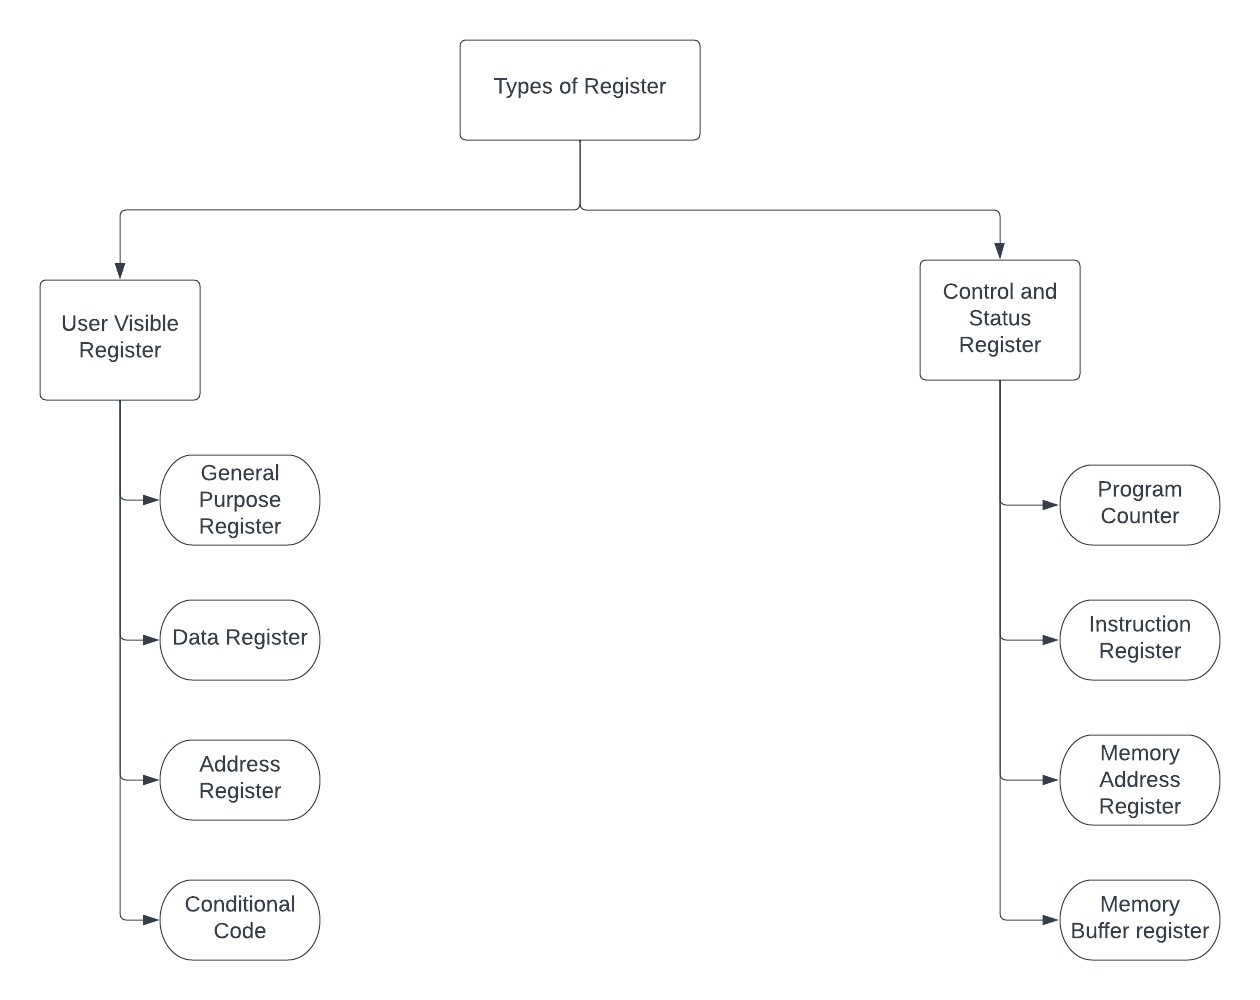
\includegraphics[scale = 0.5]{1.jpeg}
\end{center}

\section{\textbf{Data Flow Diagram Level 1:}}
\begin{center}
    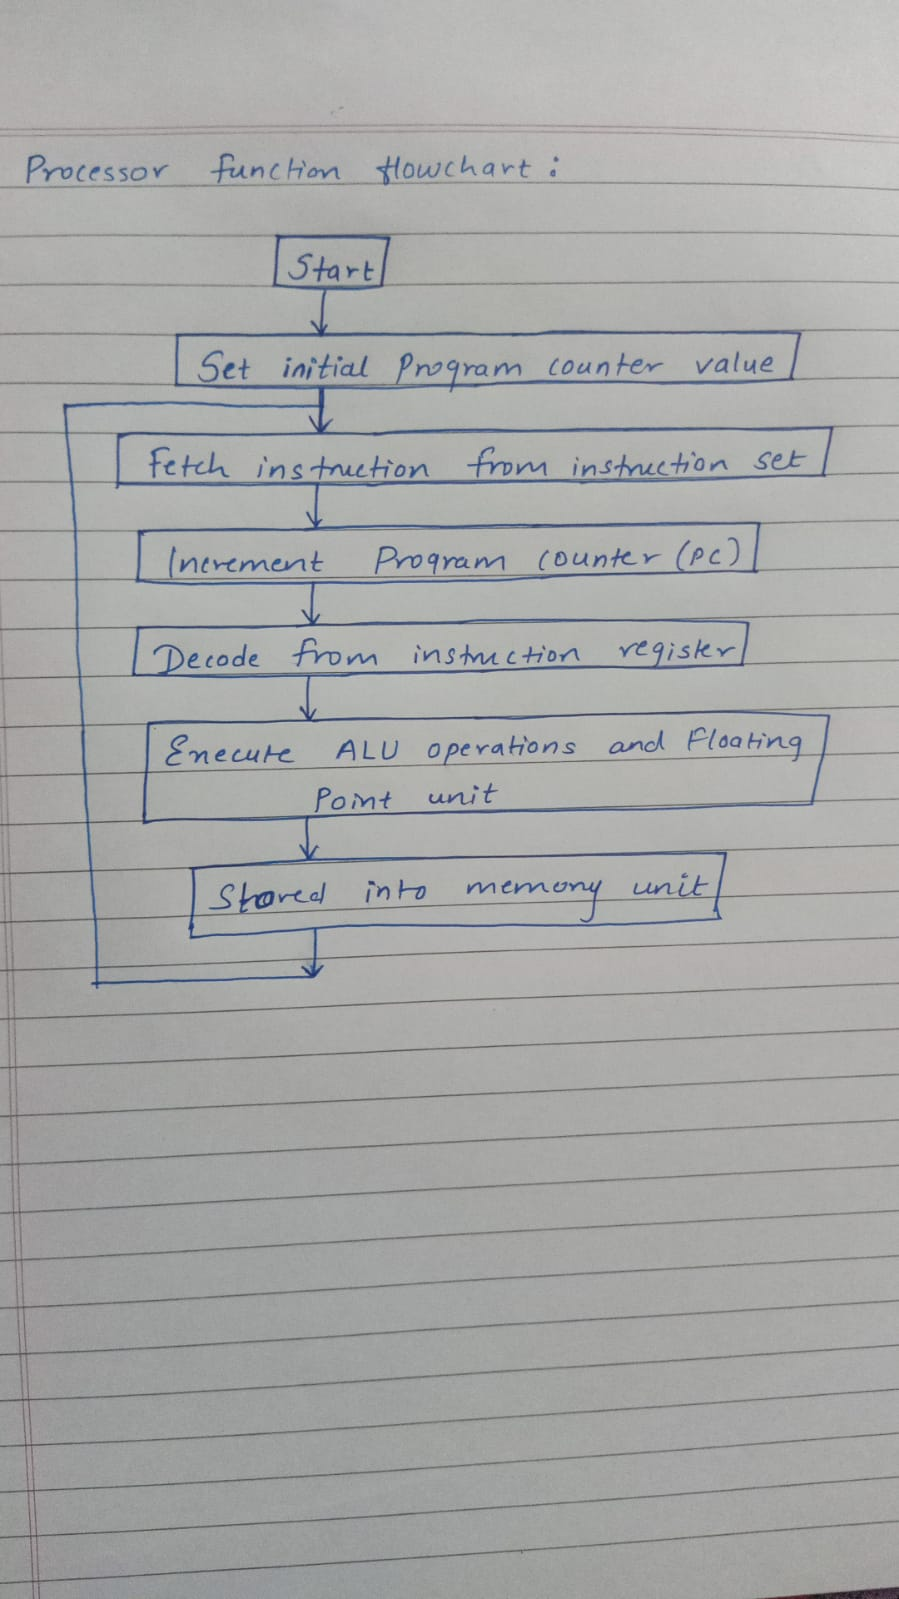
\includegraphics[scale = 0.5]{2.jpeg}
\end{center}

\section{\textbf{Data Flow Diagram Level 2:}}

\begin{center}
    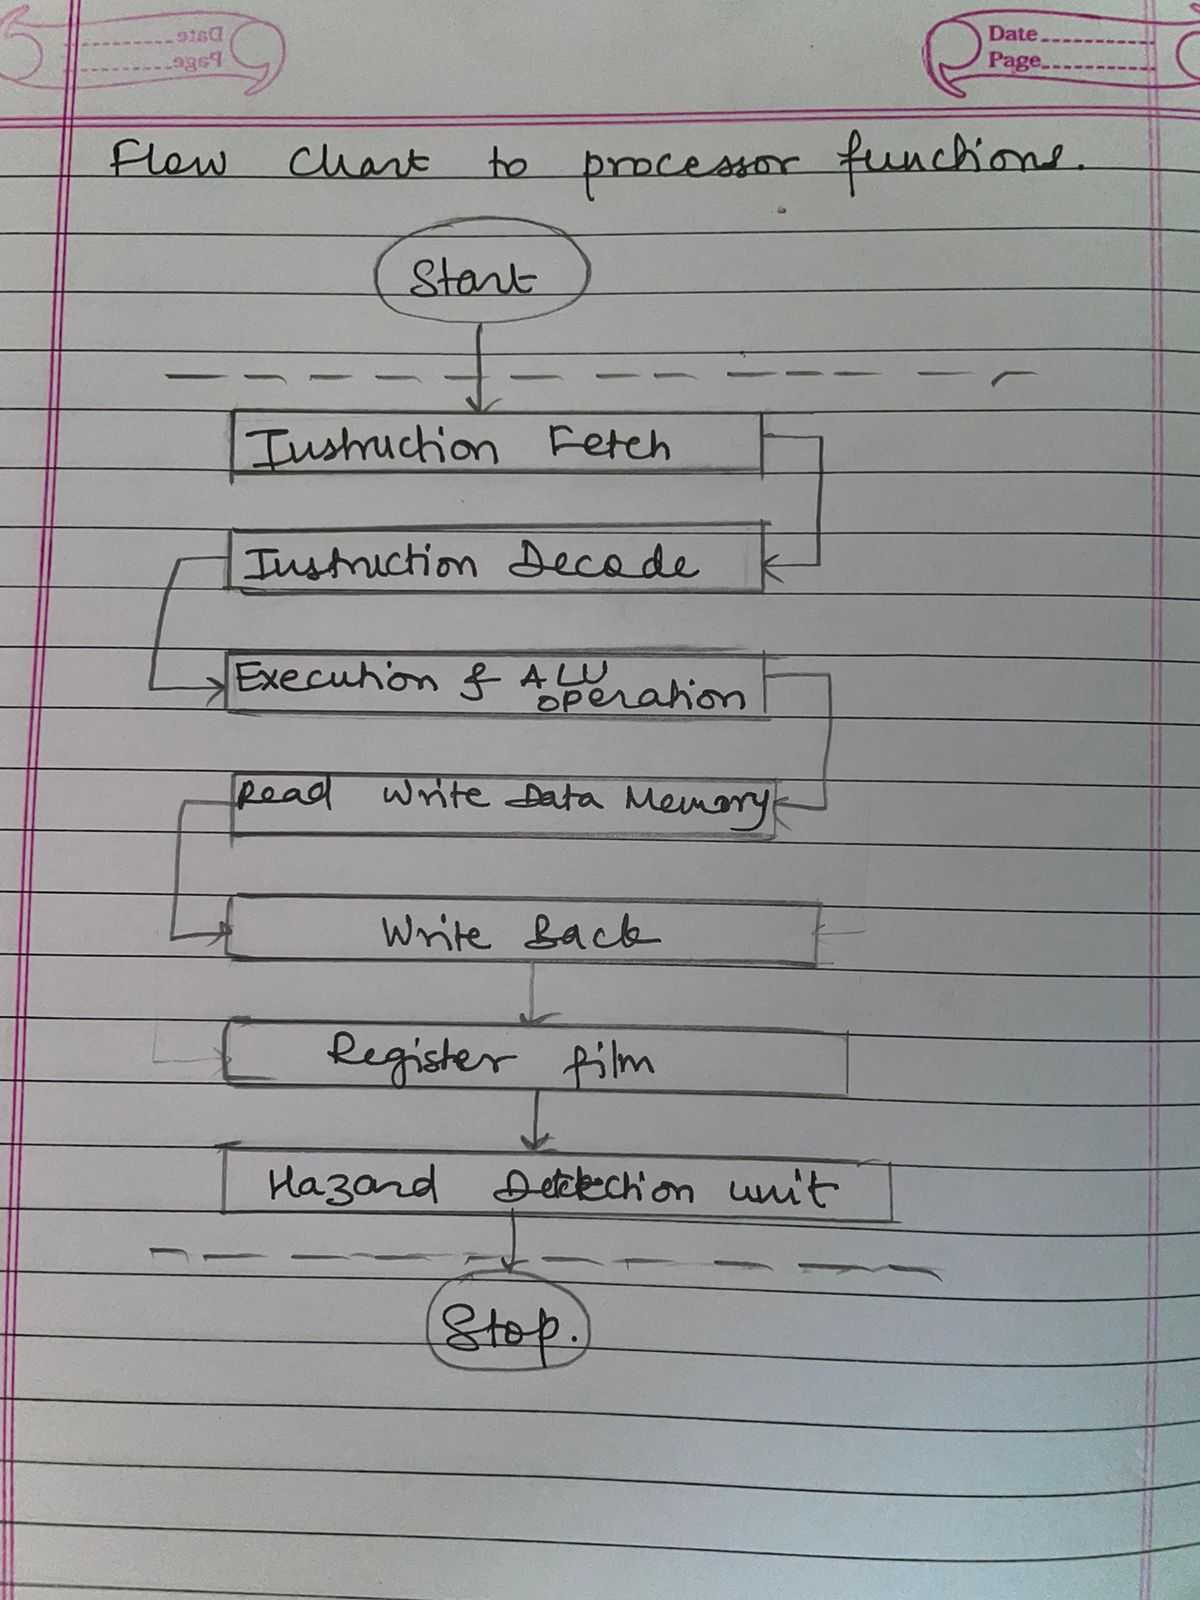
\includegraphics[scale = 0.5]{3.jpeg}
\end{center}

\section{\textbf{Conclusion:}}
Hence, learned to draw data flow diagram of level 0, level 1 ,level 2 and control flow diagram.

\section{\textbf{FAQs:}}
\subsection{\textbf{What is meant by context diagram?}}
DFD Level 0 is also called a Context Diagram. It’s a basic overview of the whole system or
process being analyzed or modeled. It’s designed to be an at-a-glance view, showing the system
as a single high-level process, with its relationship to external entities. It should be easily
understood by a wide audience, including stakeholders, business analysts, data analysts and
developers.

\subsection{\textbf{What are different levels of Data flow diagram?}}
A data flow diagram can dive into progressively more detail by using levels and layers, zeroing
in on a particular piece. DFD levels are numbered 0, 1 or 2, and occasionally go to even Level
3 or beyond. The necessary level of detail depends on the scope of what you are trying to accomplish. Level 0 is just a basic overview, Level 1 is a more detailed view, and Level 2 is the
most detailed view.

\end{document}